

\section{Objetivo}
Que el alumno comprenda la noción de \emph{Estado} y \emph{Espacio de Búsqueda}, y que pueda representar en una estructura de datos todos los posibles estados de un mundo dado. \par

\section{Introducci\'on}
Dado un problema o modelo es posible determinar las características del mundo descrito en él. Uno de los puntos a tratar es la representación de dicho mundo y el concepto de estado. Un estado es una configuración posible del mundo con el que se trabaja. Por ejemplo, un juego de ajedrez se compone de un tablero de 64 cuadros donde inicialmente están 32 piezas (16 para cada jugador). El estado inicial del ajedrez se muestra en la \fref{fig:ajedrez}.\par

\begin{figure}
  \centering
  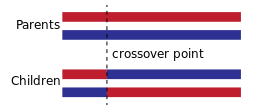
\includegraphics[width=0.4\textwidth]{estados/screen1.png}
  \caption{Estado inicial del juego de ajedrez.}
  \label{fig:ajedrez}
\end{figure}

Cuando una pieza se mueve, el estado del ajedrez cambia; pues la posición y cantidad de las piezas en juego determinan el estado del ajedrez.  De esta manera el \emph{espacio de estados} se representa como una gráfica donde cada nodo representa un estado del problema y las aristas que los unen son la aplicación de un operador o función.\par


\begin{figure}
  \centering
  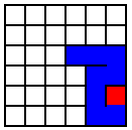
\includegraphics[width=0.9\textwidth]{estados/screen4.png}
  \caption{Ejemplo de un espacio de estados con las transiciones entre ellos. \protect\footnotemark }
  \label{fig:espacioestados}
\end{figure}

\footnotetext{Milton A. Ramírez Klapp, Notas de Inteligencia Artificial, Universidad San Sebastián, Facultad de Ingeniería y Tecnología.}

Es decir, el espacio de estados son todas las posibles configuraciones del problema. En el caso del ajedrez, las operaciones que unen cada estado en la gráfica representan el movimiento de una pieza por parte del jugador y son el otro elemento requerido para el definir el \emph{sistema de transiciones de estados}.\par


\section{Desarrollo e implementaci\'on}

La práctica consiste de generar los sucesores de los estados válidos del juego del Gato (también llamado Tres en línea).\par
Recordemos que el juego del Gato es entre dos jugadores, representados por los símbolos \enquote{\classname{X}} y \enquote{\classname{O}} que toman turnos para marcar los espacios de un tablero de 3x3.
Un jugador gana cuando logra tener una línea, ya sea horizontal, vertical o diagonal, de 3 símbolos correspondientes.\par

\begin{figure}
  \centering
  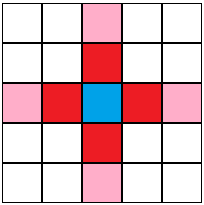
\includegraphics[width=0.7\textwidth]{estados/screen2.png}
  \caption{Ejemplo de un juego de Gato donde gana el jugador \enquote{\classname{X}}. \protect\footnotemark}
  \label{fig:tictactoe}
\end{figure}

\footnotetext{Autor: Gdr (http://en.wikipedia.org/wiki/User:Gdr)}

Afortunadamente el juego del Gato es lo bastante simple como para evitar ciclarse al generar el espacio de estados y eso es una característica importante que ayuda a la construcción del espacio de estados, ya que  podemos hacer uso de un árbol (que es un tipo especial de gráfica) para almacenar los estados.\par


\begin{figure}
  \centering
  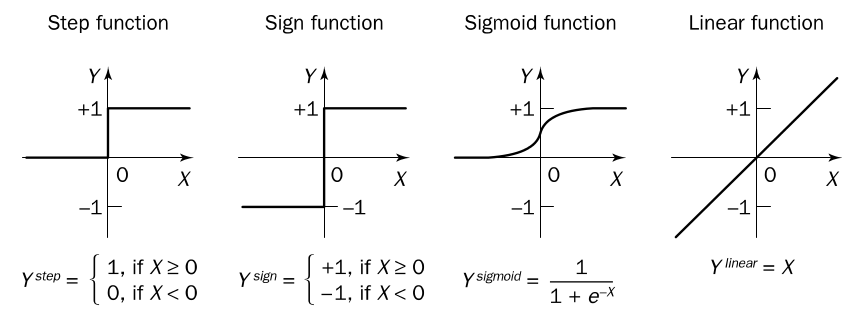
\includegraphics[width=0.8\textwidth]{estados/screen3.png}
  \caption{Espacio de búsqueda en el juego del Gato representado como un árbol.}
  \label{fig:espaciogato}
\end{figure}

Por tanto, se necesitan los siguientes elementos para representar el espacio de estados del Gato:

\begin{enumerate}
  \item \textbf{Representación del estado} \hfill\par
    Una manera de representar el estado del Gato, se usará la siguiente idea:\medskip
    
    \classname{int[][] tablero = [[0,0,1], [0,0,0], [4,4,0]]}

    \begin{figure}[h!]
      \begin{center}
        \begin{tabular}{c l | l | l }
           & \multicolumn{1}{c}{\tiny{0}} & \multicolumn{1}{c}{\tiny{1}} & \multicolumn{1}{c}{\tiny{2}} \\
           \multicolumn{1}{c}{\tiny{0}} &   &   & O \\ \cline{2-4}
           \multicolumn{1}{c}{\tiny{1}} &   &   &   \\ \cline{2-4}
           \multicolumn{1}{c}{\tiny{2}} & X & X &
        \end{tabular}
      \end{center}
      \caption{Representación gráfica del estado del Gato}
      \label{fig:representacionestado}
    \end{figure}

    Con \classname{1} representando al primer jugador y \classname{4} al segundo (fig~\ref{fig:representacionestado}).


  \item \textbf{Función generadora}\hfill \\
    Se necesitará implementar una función que genere los sucesores de un estado del juego del Gato, considerando sólo las jugadas válidas y descartando simetrías.

  \item \textbf{Función de comprobación} \hfill \\
    Se necesitará implementar una función que verifique si hubo ganador en un estado dado, utilizando una bandera para indicar que no se debe generar sucesores de ese estado, para evitar generar estados inalcanzables.
\end{enumerate}


\subsection{Implementaci\'on}
Se volverá a trabajar con \classname{Processing}.

Se debe programar lo referente a generación de sucesores de un estado, verificación de simetrías y agregar variables que lleven el conteo de empates y juegos ganados por cada jugador, esto se imprimirá junto con la información de nodos del nivel generado.

\noindent En pocas palabras es necesario implementar los siguientes métodos:

\begin{itemize}
  \item \classname{LinkedList<Gato> generaSucesores()}
  \item \classname{boolean esSimetricoDiagonalInvertida(Gato otro)}
  \item \classname{boolean esSimetricoDiagonal(Gato otro)}
  \item \classname{boolean esSimetricoVerticalmente(Gato otro)}
  \item \classname{boolean esSimetricoHorizontalmente(Gato otro)}
  \item \classname{boolean esSimetrico90(Gato otro)}
  \item \classname{boolean esSimetrico180(Gato otro)}
  \item \classname{boolean esSimetrico270(Gato otro)}
\end{itemize}

\noindent Cada método se encuentra especificado dentro del archivo \classname{Gatos.java}.


\subsection{Punto extra}
Si lo desean pueden extenderse e implementar una función de dispersión (\textit{hash}) para cada estado generado, e implementar una lista cerrada. De esta manera se evita expandir rutas que ya se habían expandido anteriormente. Podrán obtener hasta \textbf{2} puntos extras pero cuidado: ¡no es nada trivial completar este ejercicio! pues gatos que son equivalentes bajo simetrías deben ser mapeados al mismo código de dispersión.  No se sorprendan si no pueden resolver el ejercicio a la perfección.


\section{Requisitos y resultados}

Para evaluar y calificar la práctica es necesario que se implementen todos los métodos mencionados e indicados en el código, respetando implementar sólo lo que se pide (para evitar comportamientos extraños de la simulación).
Es completamente válido utilizar bibliotecas adicionales si lo consideran necesario, así como la creación y uso de sus propios métodos auxiliares si lo desean.

Deben correr su simulación de los espacios de estados del Gato sin simetrías, y después con ellas. Agreguen en su archivo \classname{readme} un pequeño párrafo detallando sus observaciones con respecto a lo anterior.

Si crean métodos auxiliares, no olviden documentar cuál es su función.

